\section{Update Sparsity and Teacher Overlap}
\label{sec:subnetworks}

This study examines how numerical representation and optimizer history affect the concentration, overlap, and direction of teacher-conditioned parameter changes. Prior work observes concentrated changes under dense distillation supervision \citep{yu2026denseupdates}. We examine the corresponding measurements in a jointly trained student.

\subsection{How concentrated are joint parameter changes?}

Write $\Delta=\theta-\theta_0$ for cumulative changes from initialization and $u=\theta_{\mathrm{after}}-\theta_{\mathrm{before}}$ for an individual optimizer step. For either change vector $z$ with $P$ coordinates, we report the fraction of parameters whose absolute change exceeds threshold $\tau$:
\begin{equation}
 f_\tau(z)=\frac{1}{P}\sum_{j=1}^{P}\mathbf 1\{|z_j|>\tau\}.
 \label{eq:active_fraction}
\end{equation}
We also report the smallest coordinate fraction accounting for 90\% of the squared change. This measures concentration without choosing an absolute threshold. Both quantities are computed separately for FP32 optimizer weights and BF16 stored model weights.

\paragraph{Joint-training comparison.}
The M-PG and M-I64-DR branches share the training settings in Appendix~\ref{app:setup}, including domain-response averaging. Figure~\ref{fig:geometry} compares cumulative changes at common updates 1, 50, 100, 250, and 500. At update 250, PG changes 5.88\% of BF16 coordinates, with 90\% of squared change in 3.01\% of coordinates. I64 changes 7.13\%, with 90\% of squared change in 3.94\%. Both joint runs concentrate their stored parameter changes in a small fraction of the model.

The corresponding FP32 nonzero fractions are 95.73\% for PG and 96.07\% for I64. Their 90\%-energy fractions are 32.94\% and 34.82\%. Thus the apparent sparsity depends strongly on which parameter representation is measured. The actual optimizer steps at update 250 change 86.35\% of FP32 coordinates for PG and 86.70\% for I64. Threshold curves and optimizer-state controls appear in Appendix~\ref{app:records}.

\begin{figure}[t]
\centering
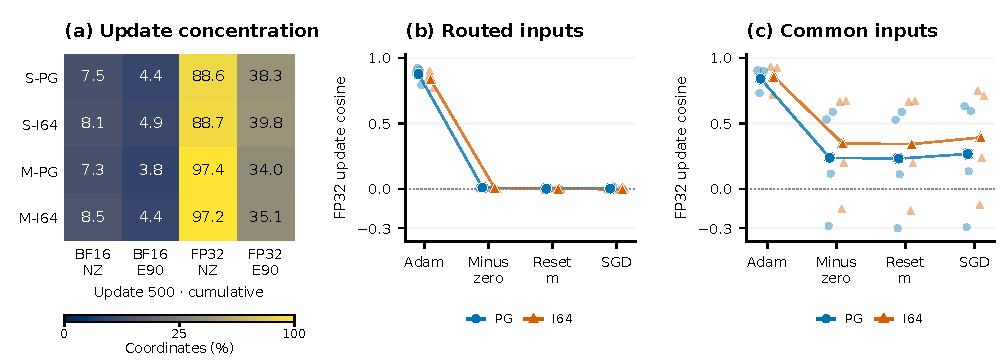
\includegraphics[width=\linewidth]{figures/nine_panel_20260914/section4_sparsity_overlap.pdf}
\caption{Parameter concentration and teacher-conditioned updates.
(a) Cumulative changes at update 500 for single-teacher (S) and joint (M) PG/I64 training, using DR. NZ is the nonzero coordinate fraction; E90 is the coordinate fraction carrying 90\% of squared change. Cells give percentages; color uses a square-root scale. S receives four times as many mathematics responses per update as M.
(b) At the common M-PG/500 student and optimizer state, FP32 top-1\% Jaccard versus signed update cosine. Small points average six teacher pairs within each bank; large points average four banks. Lines connect common-input (open) and routed-input (filled) conditions. SGD and reset-$m$ are individually norm-matched to saved-state Adam; circles denote PG and triangles I64.
(c) Teacher JS and $1-J$ on common inputs, with all six teacher pairs in all four banks. Colors and loss markers match (b); points share teachers and banks and are dependent. Updates use non-fused PyTorch steps on saved-state copies, rather than bitwise replay of the online optimizer.}
\label{fig:subnetwork_overview}
\end{figure}


\noindent Figure~\ref{fig:subnetwork_overview}(a) adds the matched single-teacher and joint cumulative measurements at update 500. The full recorded trajectories remain available in the accompanying evidence bundle.

\subsection{Do teachers change the same parameters in one student?}

Comparing teacher-specific updates requires identical copies of the joint student and its optimizer state. For teacher $d$, let $S_d(\rho)$ contain the largest-magnitude $\rho$ fraction of its parameter changes. We compare selected coordinates using Jaccard overlap:
\begin{equation}
J(d,e)=\frac{|S_d(\rho)\cap S_e(\rho)|}{|S_d(\rho)\cup S_e(\rho)|}.
\label{subnet_overlap}
\end{equation}
Equal selection sizes make the teacher pairs comparable. Overlap describes locations; the signs of the changes determine whether contributions at those locations agree. This distinction follows the support-overlap analysis of \citet{yu2026denseupdates}.

At the common M-PG/500 state, routed-input teacher updates have mean FP32 cosines of 0.8774 for PG and 0.8347 for I64 under saved-state Adam. Resetting the first moment or using norm-matched SGD brings their mean cosines close to zero (Figure~\ref{fig:subnetwork_overview}b). Each small point summarizes six teacher pairs within one of four response banks; large points average the four banks. These are local diagnostic repeats, not independent training runs. Appendix~\ref{app:completed_results} retains the joint overlap--direction and teacher-JS views, while Appendix~\ref{app:gradient_overlap} gives the separate raw-gradient input controls.

\subsection{How much alignment remains after removing the history-only step?}

Let $U(g;H)$ denote an optimizer step for current gradient $g$ at saved optimizer state $H$. We compare the complete teacher-conditioned step with its difference from the zero-current-gradient step,
\begin{equation}
\delta U_d=U(g_d;H)-U(0;H).
\label{eq:history_subtracted}
\end{equation}
This difference retains the same parameters and optimizer state in both branches. It is a nonlinear counterfactual difference, not an additive decomposition of teacher contributions.

Under routed inputs, the mean PG/I64 cosines fall to 0.0098/0.0067 after this subtraction (Figure~\ref{fig:subnetwork_overview}b). Under common inputs, they fall from 0.8415/0.8562 to 0.2373/0.3462 (panel c). The strong alignment of the complete steps therefore depends on shared optimizer history and input conditions. Routed inputs vary both teacher identity and input domain; common-input controls hold the prefixes fixed. Coordinate overlap can remain substantial even when directions differ, and neither statistic establishes the absence of cross-domain functional harm. The required teacher-by-probe-domain loss intervention is distinct from this geometric comparison.
